\documentclass[12pt, a4paper, twoside, openany]{article}

\usepackage{sectsty}
\usepackage{multirow}
\usepackage{xcolor}
\usepackage{graphicx}

\begin{document}
    \allsectionsfont{\sffamily}

    \setlength{\parindent}{0 em}
    \setlength{\parskip}{1.5 ex plus 1 ex minus 1 ex}

    \LARGE 
    \begin{center}
        \texttt{README.pdf} \textsf{for Brunn on Ubuntu}
    \end{center}
    \normalsize

    \tableofcontents

    \newpage

    \section{Usernames and passwords}
    \subsection*{Ubuntu}
    This Ubuntu installation comes with running versions of Bioclipse and
    Brunn. It has a user with \texttt{sudo} powers which you might want to
    change the password for. Here is a list of all passwords in the system: 

    \begin{center}
        \begin{tabular}{|c|l|l|}
        \hline
        Program & \multicolumn{2}{|c|}{User Credentials} \\
        \hline
        \multirow{2}{*}{Ubuntu} & username 
                                & \colorbox{yellow}{\texttt{brunn}} \\
                                & password 
                                & \colorbox{yellow}{\texttt{brunn}} \\
        \hline
        \multirow{2}{*}{MySQL}  & username 
                                & \colorbox{yellow}{\texttt{root}}  \\
                                & password 
                                & \colorbox{yellow}{\texttt{brunn}} \\
        \hline
        \end{tabular}
    \end{center}

    \subsection*{Brunn}
    There are two Brunn users created in the Brunn database.

    \begin{center}
        \begin{tabular}{|c|l|l|}
            \hline
            User type & \multicolumn{2}{|c|}{User Credentials} \\
            \hline
            \multirow{2}{*}{Administrator} 
                           & username 
                           & \colorbox{yellow}{\texttt{admin}} \\
                           & password 
                           & \colorbox{yellow}{\texttt{admin}} \\
            \hline
            \multirow{2}{*}{Standard User} 
                           & username 
                           & \colorbox{yellow}{\texttt{user}}  \\
                           & password 
                           & \colorbox{yellow}{\texttt{user}}  \\
            \hline
        \end{tabular}
    \end{center}

    \newpage

    \section{Getting started}
    Start Bioclipse from the desktop. Bioclipse should start with the Brunn
    view to the left. Double click the \texttt{Not Logged In}, or right click
    and choose \texttt{Log In}.

    \begin{center}
        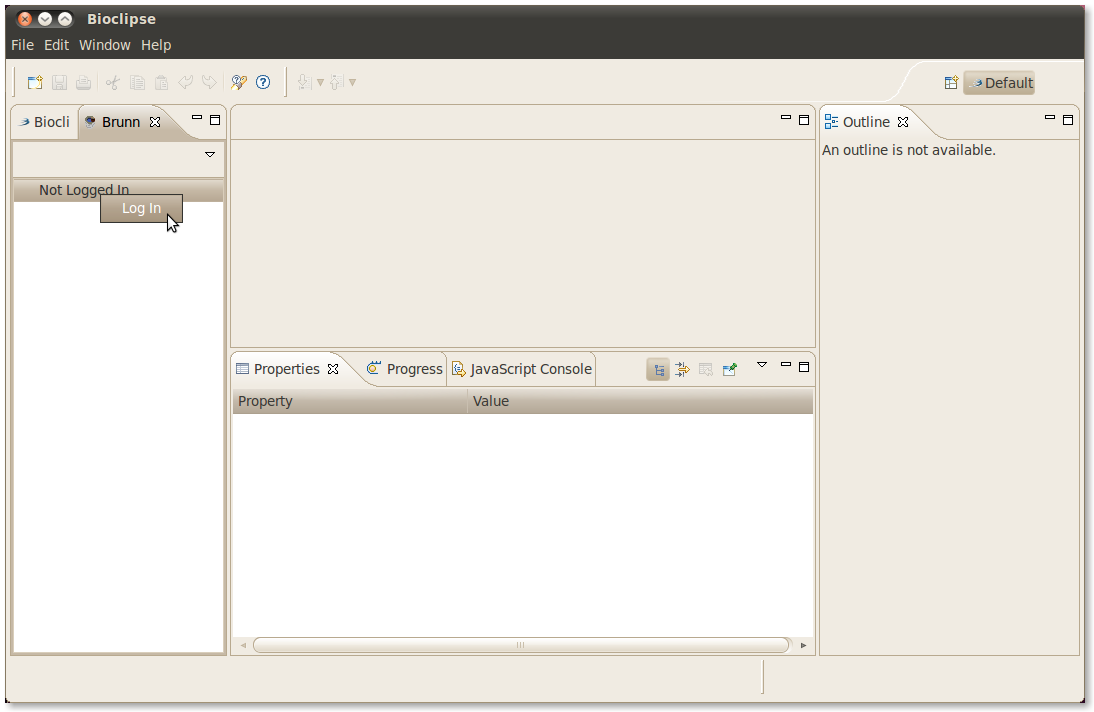
\includegraphics[scale=1.2]{images/1.png}
    \end{center}

    Log in as one of the Brunn users. For example, \texttt{user} with password
    \texttt{user}.

    \begin{center}
        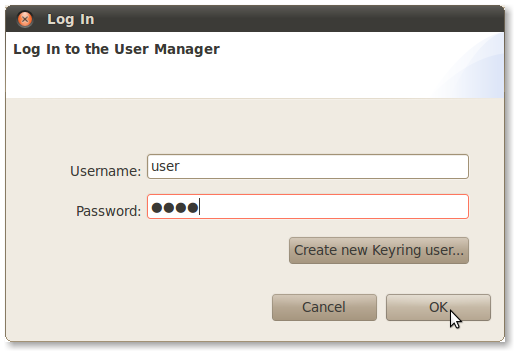
\includegraphics[scale=1.2]{images/2.png}
    \end{center}

    \newpage

    To access the Brunn help, click \texttt{Help} and then \texttt{Help
    Contents}.

    \begin{center}
        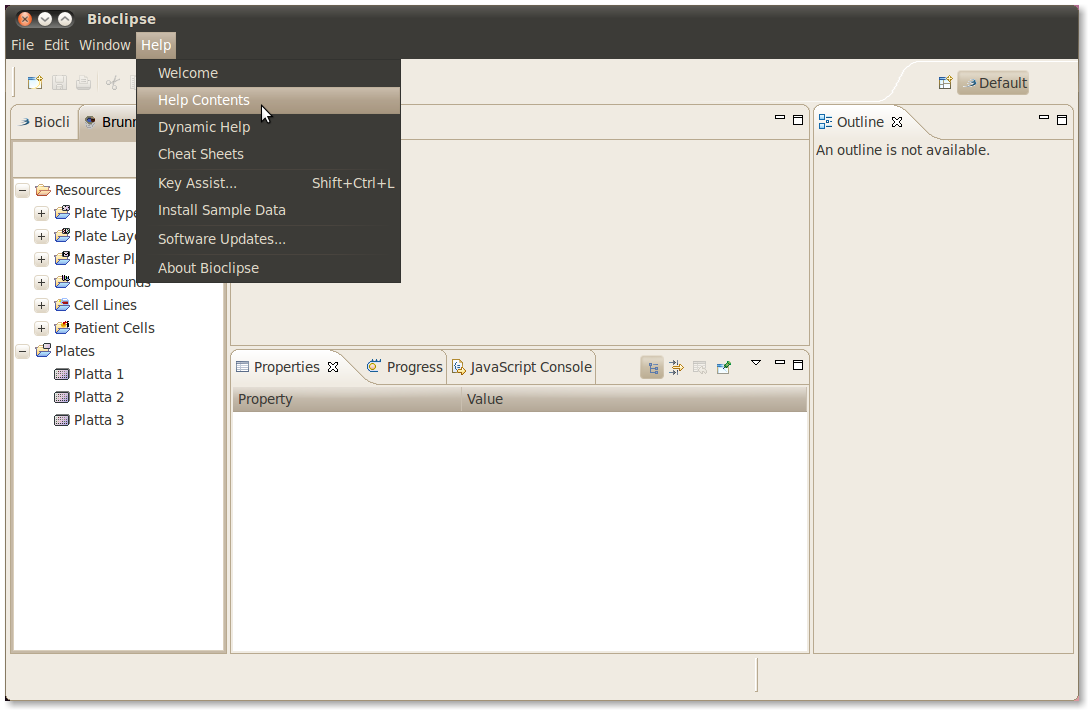
\includegraphics[scale=1.2]{images/5.png}
    \end{center}

    \begin{center}
        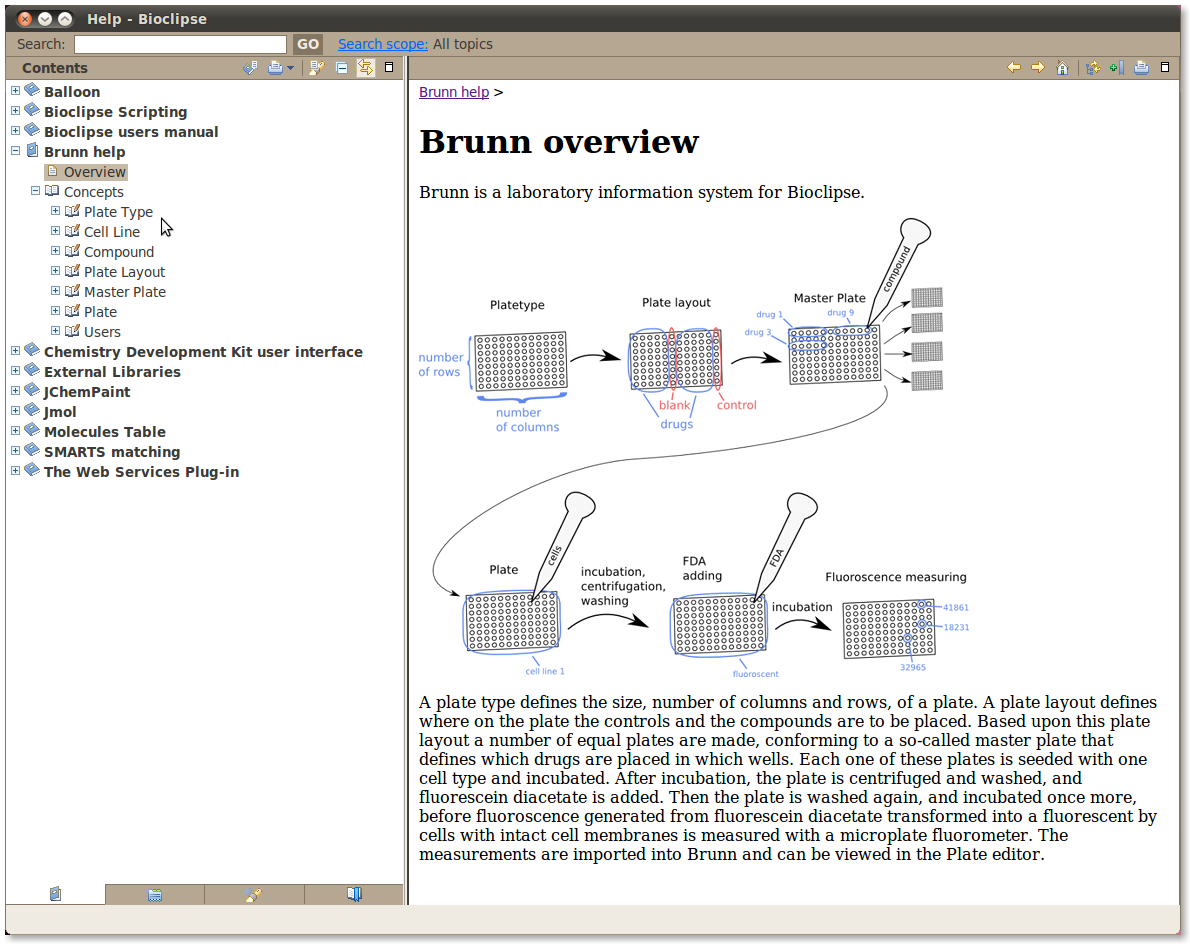
\includegraphics[scale=1.2]{images/6.png}
    \end{center}

    \newpage

    Cheat sheets are instructions for performing more specific tasks and can be
    displayed inside the Bioclipse application. To open a Brunn cheat sheet,
    click \texttt{Help} and \texttt{Cheat Sheets}, then select one of the Brunn
    cheat sheets.

    \begin{center}
        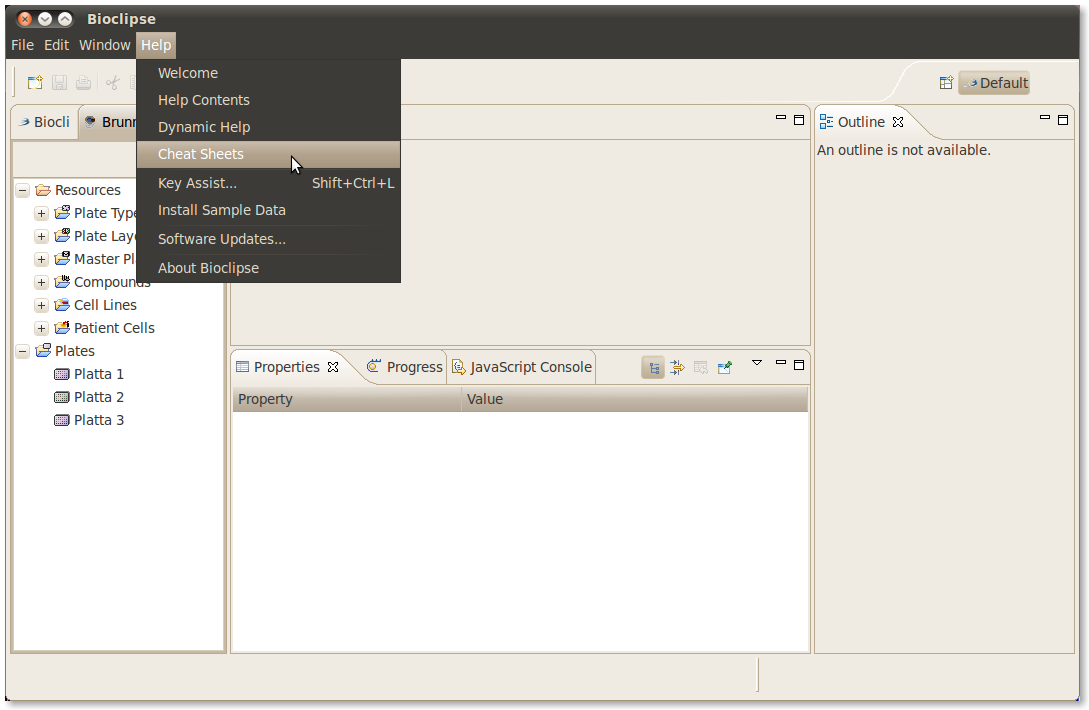
\includegraphics[height=35ex]{images/3.png}
        \hfill
        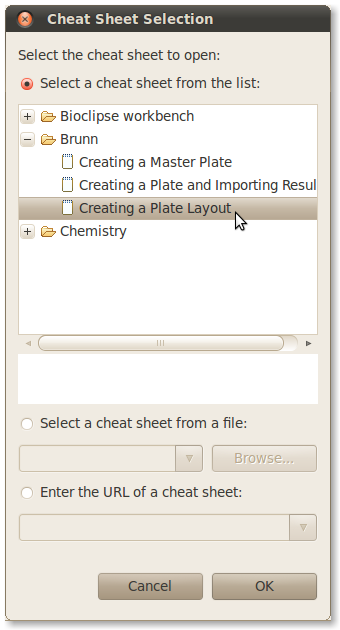
\includegraphics[height=35ex]{images/4.png}
    \end{center}

    \newpage

    \section{Examples}

    \subsection*{Example data}
    The database on this virtual box comes with a set of example plates with
    data imported for them and in the \texttt{example data} folder on the
    desktop are a series of files containing raw data for those and other
    plates. Although these files contain data from experiments and hence are
    run on some special plate layout they can of course be used as example data
    for any plates created while test running the system. During the import
    step, the barcode is read from the file but it can be changed into
    something else (\textit{e.g.} the barcode of a newly created test plate
    which a user wants to populate with data) during the import step. Just try
    importing from one of those files and then change the barcode field in the
    table, and don't forget to check the box saying that you want to import
    data for that plate.

    \begin{center}
        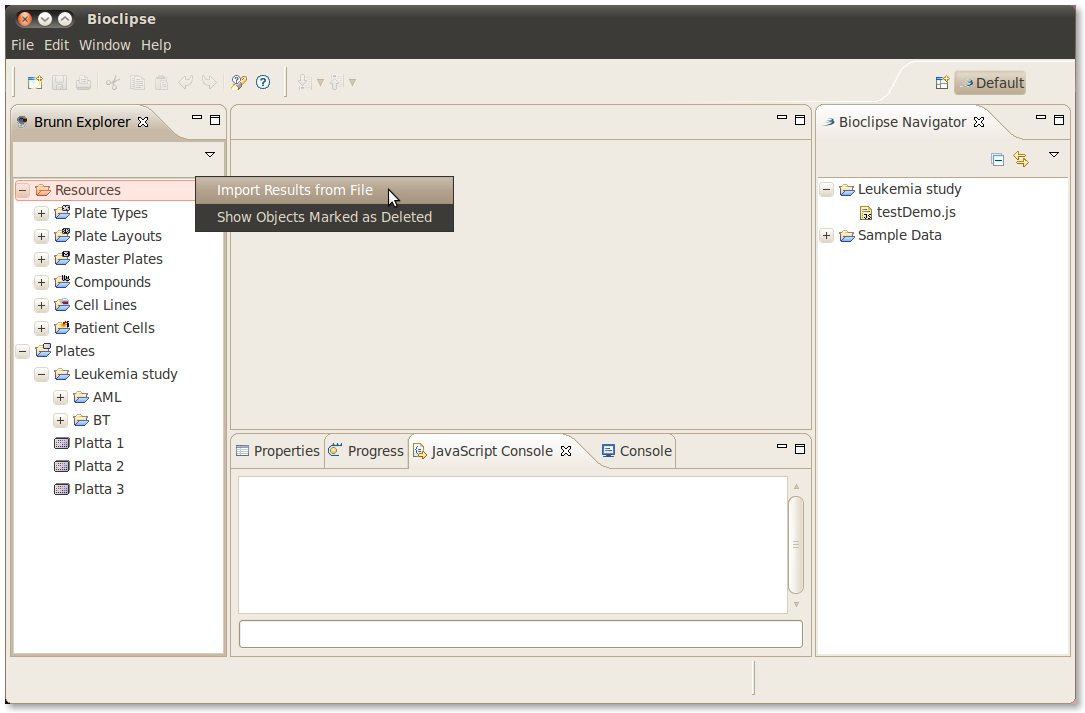
\includegraphics[scale=1.2]{images/import.png}
    \end{center}

    \begin{center}
        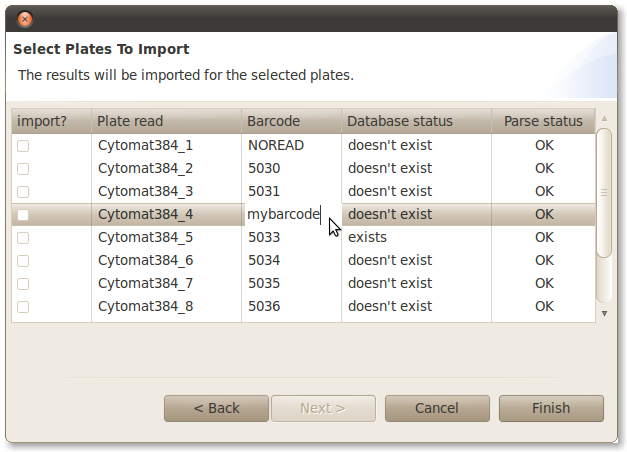
\includegraphics[scale=1.2]{images/changeBarcode.png}
    \end{center}
    \newpage

    \subsection*{Example JavaScript}
    There is also an example JavaScript \texttt{exampleDemo.js} script
    avialable which gives a taste of what can be performed from the scripting
    environment. It can be found in the \texttt{Leukemia Study} folder in the
    \texttt{Bioclipse Navigator} view.

    The \texttt{exampleDemo.js} script runs a t-test for one concentration of
    Melfalan on the two plate groups in the example data.

    \begin{center}
        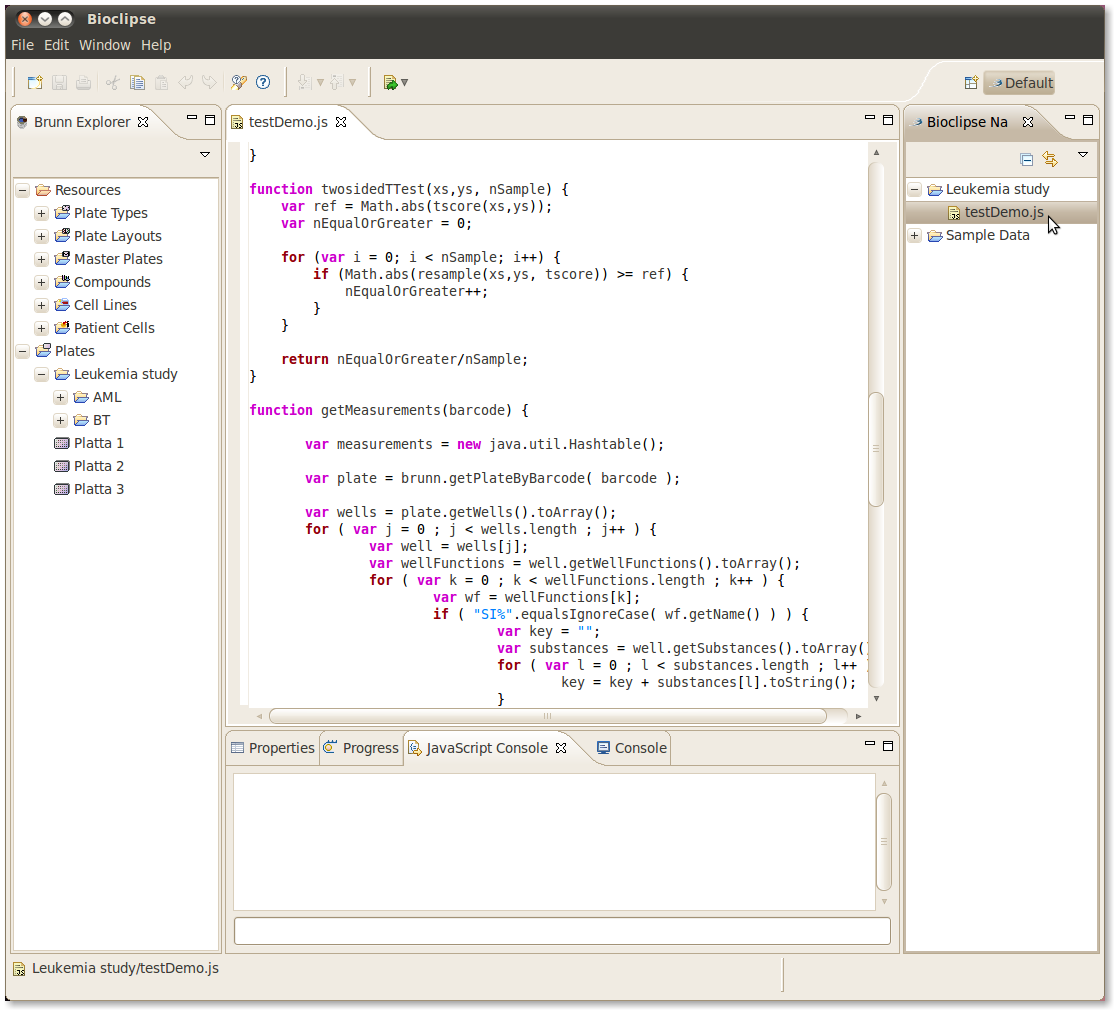
\includegraphics[scale=1.2]{images/testDemo.png}
    \end{center}

    \newpage

    \section{Updating}
    If updates are available on the update site, they can be installed by
    \texttt{Help} and \texttt{Software Updates\ldots} By default, the Updates
    dialog only lists update sites containing new versions so unless a new
    version of Brunn is available it will only show the two default Bioclipse
    update sites. If there are any desired updates on the site select to
    install them (if they have dependencies you can add those automagicly by
    clicking \texttt{Select Required}) and install them.

    \begin{center}
        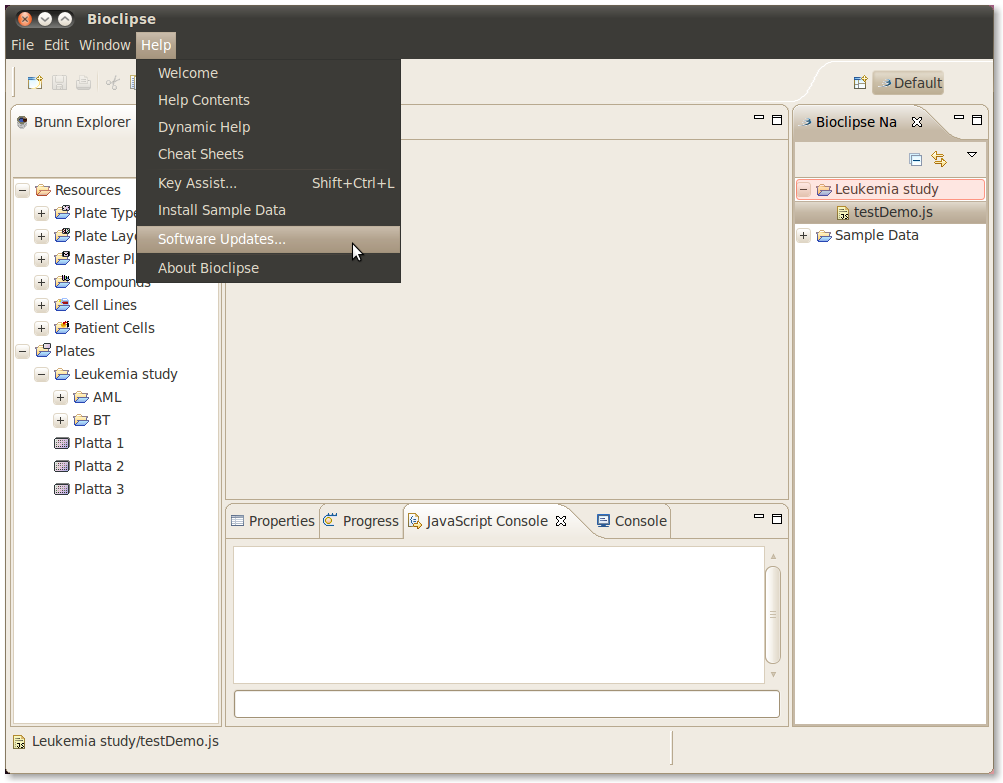
\includegraphics[scale=1.2]{images/softwareUpdates.png}
    \end{center}

    \begin{center}
        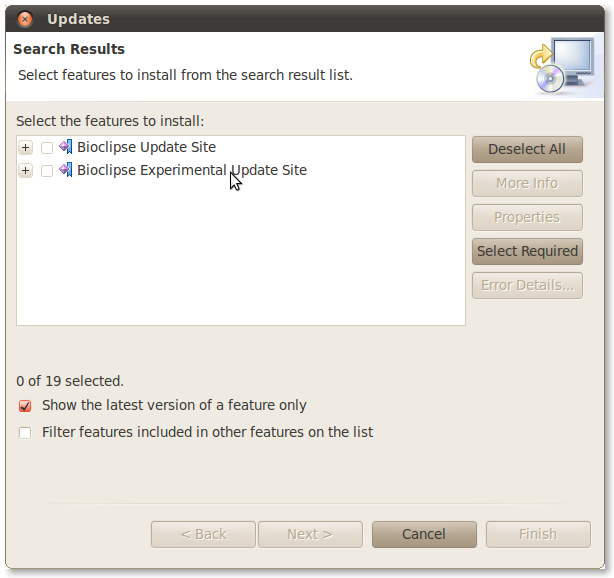
\includegraphics[scale=1.2]{images/Updates.png}
    \end{center}

\end{document}
